\documentclass{beamer}
\usepackage{../../shared/styles/custom}


%\beamerdefaultoverlayspecification{<+->}
% \newcommand{\data}{\mathcal{D}}
% \newcommand\Item[1][]{%
% 	\ifx\relax#1\relax  \item \else \item[#1] \fi
% 	\abovedisplayskip=0pt\abovedisplayshortskip=0pt~\vspace*{-\baselineskip}}

\graphicspath{ {../assets/shuffling/figures/} }



\title{Shuffling}
\date{\today}
\author{Nipun Batra}
\institute{IIT Gandhinagar}
\begin{document}
	\maketitle

	\begin{frame}{Consider this dataset}
		First 80 examples are of class ``Yes"\\
		Remaining 20 examples are of class ``No".
		\begin{table}[]
		\centering
		\begin{tabular}{|c|c|c|}
		\hline
		\textbf{\begin{tabular}[c]{@{}c@{}}Serial\\ Number\end{tabular}} & \textbf{...} & \textbf{Class} \\ \hline
		1 &  & Yes \\ \hline
		2 &  & Yes \\ \hline
		3 &  & Yes \\ \hline
		\begin{tabular}[c]{@{}c@{}}.\\ .\end{tabular} &  & \begin{tabular}[c]{@{}c@{}}.\\  .\end{tabular} \\ \hline
		80 &  & No \\ \hline
		81 &  & No \\ \hline
		\begin{tabular}[c]{@{}c@{}}.\\ .\end{tabular} &  & \begin{tabular}[c]{@{}c@{}}.\\ .\end{tabular} \\ \hline
		100 &  & No \\ \hline
		\end{tabular}
		\end{table}
	\end{frame}
	
	\begin{frame}{Consider this dataset}
	\only<1->{
		While using a 80-20 train-test split , we will get the distribution shown below
		\vspace{0.5cm}
		\begin{center}
		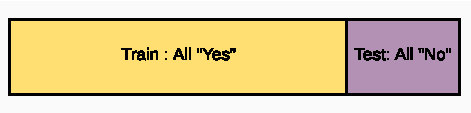
\includegraphics[]{img1}
		\end{center}
	}
	\only<2->{
	Will we learn anything useful in this scenario?
	}
	\only<3->{
		$No $ :(\\
		\vspace{1cm}
	}
	
	\only<4->{$Solution$ : Shuffle before learning}	

	\end{frame}	

	\begin{frame}{Why shuffle for SGD?}
		\only<1->
		{
			We can fall into a loop!\\
			\vspace{1cm}
			SGD on point 1 : $\theta_0 + 0.2, \theta_1 - 0.2$\\
			SGD on point 2 : $\theta_0 - 0.2, \theta_1 + 0.2$\\
			\vspace{1cm}
			Biased learning as point 2 follows point 1.
		}
		
	\end{frame}

\end{document}
